\documentclass[a4paper, 12pt]{article}

% -- Language --
\usepackage[spanish]{babel}
\usepackage[utf8]{inputenc}

% ----- Fonts -----
% -- Fuente --
% \usepackage{fontspec}
% \setmonofont{JetBrainsMono Nerd Font}  

% -- Color --
\usepackage{xcolor}
%\definecolor{azul}{RGB}{00,33,99}
\definecolor{azul}{RGB}{35,72,180}

% -- Page Margin --
\usepackage[margin=1in]{geometry}

% -- Espaciados --
\newcommand{\Pspace}{0.5cm}
\newcommand{\Aspace}{0.2cm}

% -- Columnas --
\usepackage{multicol}

% -- Imagenes --
\usepackage{graphicx}
\usepackage{float}

% -- Matemáticas --
\usepackage{amsmath, amssymb}

% -- Gráficas --
\usepackage{pgfplots}
\pgfplotsset{compat=1.18}

% -- Código --
\usepackage{listings}
\lstset{
    language=C++,                   % Lenguaje del código
    basicstyle=\ttfamily\small,     % Fuente del código
    keywordstyle=\color{blue},      % Color de palabras clave
    commentstyle=\color{gray},      % Color de comentarios
    stringstyle=\color{red},        % Color de cadenas
    numbers=left,                   % Números de línea a la izquierda
    numberstyle=\tiny\color{gray},
    breaklines=true,                % Permitir saltos de línea
    frame=single                    % Marco alrededor del código
}



\title
{
    Diseño de Sistemas Digitales 2025-2 \\
    Problemas Unidad 3
}

    \begin{document}

    \maketitle

    \begin{center}
        \begin{tabular}{r|l}
            \textbf{Expediente} & \textbf{Nombre} \\ \hline
            219208106 & Bórquez Guerrero Angel Fernando \\
        \end{tabular}
    \end{center}

    \rule{\linewidth}{0.3mm}



    \vspace{0.3cm}
    \begin{enumerate}
        % - Problema 1
        \item Simplifique las siguientes expresiones mediante el uso del álgebra booleana. \par
             % Respuestas:
            \vspace{\Aspace} \par
            a) $x = ABC + \bar{A}C$
            \\ { \color{azul} 
                $C(AB + \bar{A})$
                \par $C(B + \bar{A})$
            }

            \vspace{\Aspace} \par
            b) $y = (Q + R)(\bar{Q} + \bar{R})$
            \\ { \color{azul} 
                $Q\bar{Q} + Q\bar{R} + \bar{Q}R + R\bar{R}$
                \par $Q\bar{R} + \bar{Q}R$
            }

            \vspace{\Aspace} \par
            c) $w = ABC + A\bar{B}C + \bar{A}$
            \\ { \color{azul} 
                $AC(B + \bar{B}) + \bar{A}$
                \par $AC + \bar{A}$
                \par $C + \bar{A}$
            }

            \vspace{\Aspace} \par
            d) $q = \overline{RST}\overline{(R + S + T)}$
            \\ { \color{azul} 
                $(\bar{R} + \bar{S} + \bar{T})(\bar{R}\bar{S}\bar{T})$
                \par $\bar{R}(\bar{R}\bar{S}\bar{T}) + \bar{S}(\bar{R}\bar{S}\bar{T}) + \bar{T}(\bar{R}\bar{S}\bar{T})$
                \par $\bar{R}\bar{S}\bar{T} + \bar{R}\bar{S}\bar{T} + \bar{R}\bar{S}\bar{T}$
                \par $\bar{R}\bar{S}\bar{T}$
            }

            \vspace{\Aspace} \par
            e) $x = \bar{A}\bar{B}\bar{C} + \bar{A}BC + ABC + A\bar{B}\bar{C} + A\bar{B}C$
            \\ { \color{azul} 
                $\bar{B}\bar{C}(\bar{A} + A) + BC(\bar{A} + A) + A\bar{B}C$
                \par $\bar{B}\bar{C} + BC + A\bar{B}C$
                \par $\bar{B}\bar{C} + C(B + A \bar{B})$
                \par $\bar{B}\bar{C} + C(B + A)$
            }

            \newpage
            \vspace{\Aspace} \par
            f) $z = (B + \bar{C})(\bar{B} + C) + \overline{\bar{A} + B + \bar{C}}$
            \\ { \color{azul} 
                $(B + \bar{C})(\bar{B} + C) + A\bar{B}C$
                \par $B\bar{B} + \bar{B}\bar{C} + BC + C\bar{C} + A\bar{B}C$
                \par $\bar{B}\bar{C} + BC + A\bar{B}C$
                \par $\bar{B}(\bar{C} + AC) + BC$
                \par $\bar{B}(\bar{C} + A) + BC$
            }



        % - Problema 2
        \vspace{\Pspace}
        \item Simplifique el circuito de la figura mediante el uso del álgebra booleana. \par
        \begin{figure}[!ht]
            \centering
            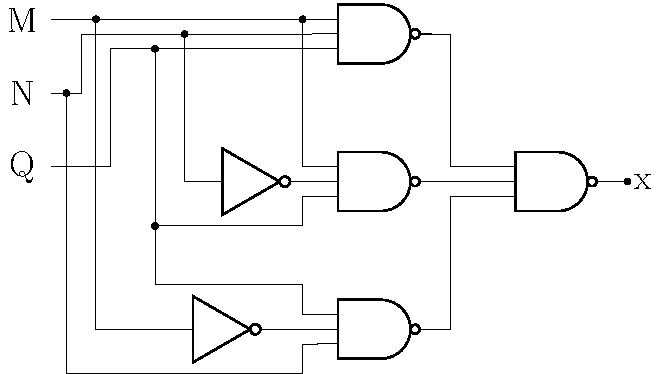
\includegraphics[width=0.7\textwidth]{Circuitos/Figuras/Figura-2.pdf}
        \end{figure}
            % Respuesta:
            \vspace{\Aspace} \par
            { \color{azul} Expresión: $\overline{(\overline{(MNQ)} \text{ } \overline{(M\bar{N}Q)} \text{ } \overline{(\bar{M}NQ)})}$
                \par $MNQ + M\bar{N}Q + \bar{M}NQ$
                \par $MQ(N + \bar{N}) + \bar{M}NQ$
                \par $MQ + \bar{M}NQ$
                \par $Q(M + \bar{M}N)$
                \par $Q(M + N)$
                \begin{figure}[!ht]
                    \centering
                    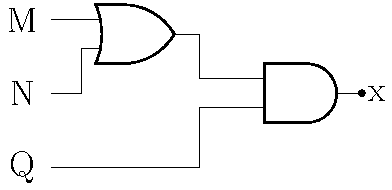
\includegraphics[width=0.5\textwidth]{Circuitos/Respuestas/Respuesta-2.pdf}
                \end{figure}
            }



        \newpage
        % - Problema 3
        \item Diseñe el circuito lógico que corresponde a la tabla de verdad que se muestra a continuación:
        \begin{center}
            \begin{tabular}{ccc|c}
                \textbf{A} & \textbf{B} & \textbf{C} & \textbf{x} \\
                \hline
                0 & 0 & 0 & 1 \\
                0 & 0 & 1 & 0 \\
                0 & 1 & 0 & 1 \\
                0 & 1 & 1 & 1 \\
                1 & 0 & 0 & 1 \\
                1 & 0 & 1 & 0 \\
                1 & 1 & 0 & 0 \\
                1 & 1 & 1 & 1
            \end{tabular}
        \end{center}
            % Respuesta:
            \vspace{\Aspace} \par
            { \color{azul} 
                $x = \bar{A}\bar{B}\bar{C} + \bar{A}B\bar{C} + \bar{A}BC + A\bar{B}\bar{C} + ABC$
                \par $x = \bar{A}\bar{C}(\bar{B} + B) + BC(\bar{A} + A) + A\bar{B}\bar{C}$
                \par $x = \bar{A}\bar{C} + BC + A\bar{B}\bar{C}$
                \par $x = \bar{C}(\bar{A} + A\bar{B}) + BC$
                \par $x = \bar{C}(\bar{A} + \bar{B}) + BC$
                \begin{figure}[!ht]
                    \centering
                    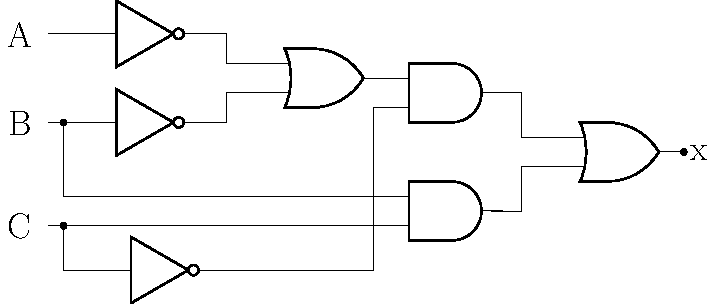
\includegraphics[width=0.7\textwidth]{Circuitos/Respuestas/Respuesta-3.pdf}
                \end{figure}
            }



        % - Problema 4
        \vspace{\Pspace}
        \item Diseñe un circuito lógico cuya salida esté en ALTO sólo cuando la mayoría de las entradas A, B y C estén en BAJO.
            % Respuesta:
            \vspace{\Aspace} \par
            { \color{azul} 
                \begin{figure}[!ht]
                    \centering
                    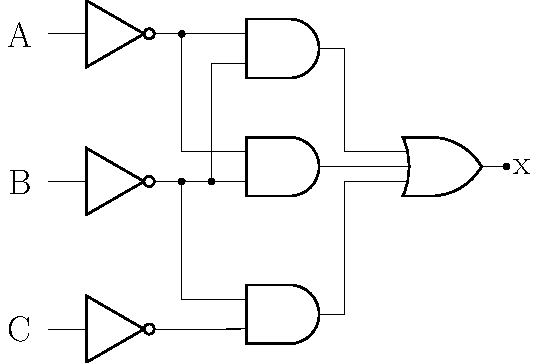
\includegraphics[width=0.5\textwidth]{Circuitos/Respuestas/Respuesta-4.pdf}
                \end{figure}
            }



        \newpage
        % - Problema 5
        \item Determine la expresión mínima para cada uno de los mapas K en la figura. \par
            % Respuestas:
            \vspace{\Aspace} \par
            a) 
            \begin{tabular}{ccccc}
                & $\bar{C}\bar{D}$ & $\bar{C}D$ & $CD$ & $C\bar{D}$ \\
                $\bar{A}\bar{B}$ & 1 & 1 & 1 & 1 \\
                $\bar{A}B$ & 1 & 1 & 0 & 0 \\
                $AB$ & 0 & 0 & 0 & 1 \\
                $A \bar{B}$ & 0 & 0 & 1 & 1
            \end{tabular}

            \par { \color{azul} 
                $\bar{A}\bar{B} + \bar{A}B\bar{C} + AC\bar{D} + A\bar{B}C$
                \par $\bar{A}(\bar{B} + B\bar{C}) + AC(\bar{D} + \bar{B})$
                \par $\bar{A}(\bar{B} + \bar{C}) + AC(\bar{D} + \bar{B})$
            }

            \vspace{\Aspace} \par
            b) 
            \begin{tabular}{ccccc}
                & $\bar{C}\bar{D}$ & $\bar{C}D$ & $CD$ & $C\bar{D}$ \\
                $\bar{A}\bar{B}$ & 1 & 0 & 1 & 1 \\
                $\bar{A}B$ & 1 & 0 & 0 & 1 \\
                $AB$ & 0 & 0 & 0 & 0 \\
                $A \bar{B}$ & 1 & 0 & 1 & 1
            \end{tabular}

            \par { \color{azul} 
                $\bar{A}\bar{C}\bar{D} + \bar{A}\bar{B}C + \bar{A}C\bar{D} + \bar{B}\bar{C}\bar{D} + A\bar{B}C$
                \par $\bar{A}\bar{D}(\bar{C} + C) + \bar{B}C(\bar{A} + A) + \bar{B}\bar{C}\bar{D}$
                \par $\bar{A}\bar{D} + \bar{B}C + \bar{B}\bar{C}\bar{D}$
                \par $\bar{A}\bar{D} + \bar{B}(C + \bar{C}\bar{D})$
                \par $\bar{A}\bar{D} + \bar{B}(C + \bar{D})$
            }



        % - Problema 6
        \vspace{\Pspace}
        \item Empezando con la tabla de verdad del problema 3, utilizce un mapa K para encontrar la ecuación SOP más simple.
            % Respuesta:
            \vspace{\Aspace} \par
            { \color{azul} 
               \begin{tabular}{ccc}
                    & $C$ & $\bar{C}$ \\
                    $\bar{A}\bar{B}$ & 0 & 1 \\
                    $\bar{A}B$ & 1 & 1 \\
                    $AB$ & 1 & 0 \\
                    $A \bar{B}$ & 0 & 1
                \end{tabular}
                
                \par $\bar{A}\bar{C} + BC + \bar{B}\bar{C}$
                \par $\bar{C}(\bar{A} + \bar{B}) + BC$
            }

            

        \newpage
        % - Problema 7
        \item Simplifique la expresión utilizando un mapa K.
            % Respuestas:
            \vspace{\Aspace} \par
            a) $x = ABC + \bar{A}BC$
            \par { \color{azul}
                \begin{tabular}{ccc}
                    & $C$ & $\bar{C}$ \\
                    $\bar{A}\bar{B}$ & 0 & 0 \\
                    $\bar{A}B$ & 1 & 0 \\
                    $AB$ & 1 & 0 \\
                    $A \bar{B}$ & 0 & 0
                \end{tabular}
            }

            \vspace{\Aspace} \par
            b) $x = \bar{A}\bar{B}\bar{C} + \bar{A}BC + ABC + A\bar{B}\bar{C} + A\bar{B}C$
            \par { \color{azul}
                \begin{tabular}{ccc}
                    & $C$ & $\bar{C}$ \\
                    $\bar{A}\bar{B}$ & 0 & 1 \\
                    $\bar{A}B$ & 1 & 0 \\
                    $AB$ & 1 & 0 \\
                    $A \bar{B}$ & 1 & 1
                \end{tabular}
            }



        % - Problema 8
        \vspace{\Pspace}
        \item Determine las condiciones de entrada necesarias para producir $x = 1$ en la figura.
        \begin{figure}[!ht]
            \centering
            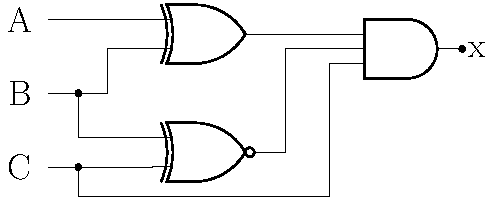
\includegraphics[width=0.7\textwidth]{Circuitos/Figuras/Figura-8.pdf}
        \end{figure}
            % Respuesta:
            \vspace{\Aspace} \par
            { \color{azul} 
                Expresión:
                \par $((A + B)(\bar{A} + \bar{B}))\overline{((B + C)(\bar{B} + \bar{C}))}C$
                \par $((A + B)(\bar{A} + \bar{B}))((\bar{B}\bar{C} + (BC))C$

                \vspace{\Aspace}
                \par Condiciones necesarias:
                \par $A = 0$, $B = 1$ y $C = 1$
            }
    \end{enumerate}
\end{document}
